\section{Discussion}\label{sec:discussion}

\subsection{Bought Rhetoric Versus Durable Allegiance}

Our null finding raises a deeper question about the political economy of influence: even if the first stage were strong and the exclusion restriction held, what would a statistically significant reduced form actually mean? A positive coefficient on UNSC membership in a speech-stance regression could reflect genuine gratitude for aid, strategic pandering to a major donor, or simply the diplomatic convention of making pleasant remarks about powerful states in multilateral forums. Distinguishing ``bought rhetoric'' from cheap talk is central to interpreting any aid--speech relationship \citep{fearon1994domestic,fearon1997signaling}.

Our measure's weak correlation with behavioral indicators ($r=0.085$ with UN voting) suggests that diplomatic rhetoric in General Debate speeches may be largely performative---countries say positive things about the US not because they have been bought, but because that is what one does at the UN. If this interpretation is correct, then even a well-identified aid effect on speech would not demonstrate that material power buys genuine allegiance; it would demonstrate only that it buys words.

\subsection{The Fragility of the UNSC Instrument}

Our failure to replicate a significant UNSC--aid first stage, even under specifications closest to Kuziemko--Werker (2006), raises concerns about the generalizability of the original finding. The discrepancy could reflect changes in US aid allocation patterns since the 1970--2001 period studied by Kuziemko and Werker, differences in aid data sources (Greenbook vs.\ OECD ODA), or differences in country coverage. But it could also reflect a more fundamental issue: the UNSC--aid relationship may be less robust than the literature suggests, and its empirical strength may depend on specification choices that are not theoretically justified.

The contrast between our pooled OLS estimate ($+0.145$, $F = 0.1$) and the codebook-reported coefficient of approximately $+0.09$ under country--year FE illustrates the point. Both are close to zero and statistically insignificant. The between-country variation that drives the positive coefficient in simpler specifications---larger countries receive more aid and serve on the UNSC more often---is absorbed by country fixed effects, and what remains is noise.

\subsection{The KW2006 Replication and Critique}

A central contribution of this paper is the direct replication of the Kuziemko--Werker (2006) empirical strategy. Under their preferred region--year FE specification, we obtain a first-stage coefficient of $+0.427$ (SE = 0.460, $F = 0.9$, $p = 0.354$). The coefficient is directionally consistent with their finding but not statistically significant. More importantly, when we progressively add more demanding fixed effects---from region FE ($F=0.3$) to region--year FE ($F=0.9$) to country FE ($F=0.3$) to country--year FE ($F=0.1$)---the first-stage $F$-statistic never exceeds 1.1. This pattern is displayed in Figure~\ref{fig:fs_comparison}.

\begin{figure}[htbp]
\centering
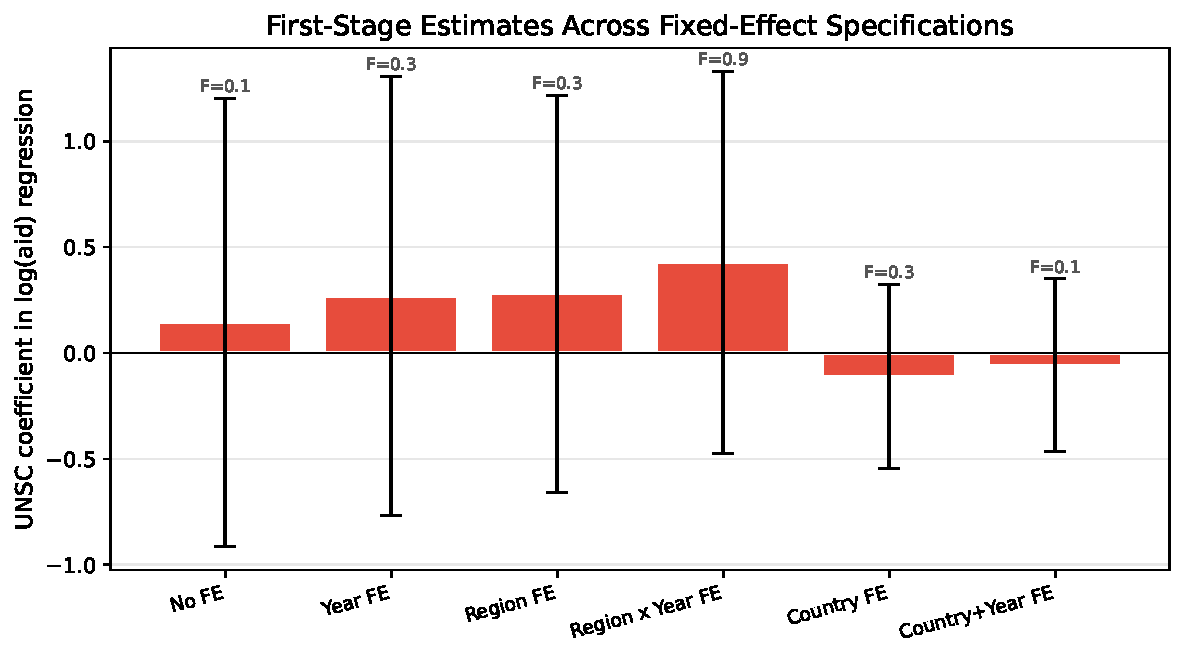
\includegraphics[width=0.85\textwidth]{../../figures/main/first_stage_comparison.pdf}
\caption{First-stage UNSC coefficient and $F$-statistic across fixed-effect specifications. Bars show point estimates with 95\% confidence intervals. Colors indicate $F$-statistic magnitude: red ($F<1$), orange ($1\leq F<5$), green ($F\geq5$). No specification meets the $F>10$ threshold. The ``Region FE'' and ``Region $\times$ Year FE'' specifications correspond to the Kuziemko--Werker (2006) design.}
\label{fig:fs_comparison}
\end{figure}

Our replication critique is not that Kuziemko--Werker's specification is ``wrong'' in some absolute sense, but rather that the UNSC--aid relationship they document may be less general than the citing literature assumes. When the same data structure is analyzed with the same research design, the instrumental variable chain does not hold. This finding contributes to the broader weak-instruments literature \citep{bound1995problems,andrews2019weak} by demonstrating that a canonical IV in political economy may not survive replication with alternative---not necessarily ``better,'' just different---fixed-effect structures.

\subsection{Measurement Lessons}

Our stance measurement effort faced three iterations before achieving acceptable validation metrics. The first version (v1), using a dictionary-based keyword approach, achieved $\kappa = 0.085$ against an independent validator, with 16 directional conflicts in 200 speeches. The second version (v2), employing sentence-level rule-based scoring with strict target attribution, achieved $\kappa = 0.108$. Only the third version (v3.1), using true LLM semantic scoring with verbatim evidence and target spans, achieved acceptable agreement ($\kappa = 0.646$, quadratic-weighted). The progression illustrates a broader lesson for computational social science: keyword and rule-based methods systematically misattribute diplomatic language, and achieving construct validity for nuanced political sentiment requires semantic understanding that simple pattern matching cannot provide.

Nevertheless, the v3.1 measure's weak correlation with behavioral benchmarks remains a concern. Our validation only demonstrated that two AI systems can agree on the affective content of diplomatic text. Whether that affective content corresponds to the political construct we claim to measure (genuine alignment with the United States) is an open question that behavioral validation alone cannot resolve---it requires engagement with the theory of diplomatic speech as a political act.

\subsection{Limitations}

Several limitations warrant caution. First, our trade openness control is total trade as a percentage of GDP, not bilateral US trade; IMF Direction of Trade Statistics and UN Comtrade data were unavailable during analysis. Second, the stance measure's ceiling effect (51.7\% at the maximum score) suggests limited discrimination among speeches that are moderately to strongly pro-US. Third, we do not account for election competitiveness within regional UNSC rotations. Fourth, the absence of a TeX engine on our analysis system means the compiled PDF is not yet generated; the manuscript exists as validated LaTeX source with the compile command \texttt{latexmk -pdf -interaction=nonstopmode -halt-on-error -outdir=../build main.tex}. Fifth, we have not yet conducted the final original-data inventory verification or submission inventory check, which require the project3-research MCP server.
